\documentclass[handout]{beamer}
\usepackage[utf8]{inputenc} 
\usepackage[T1]{fontenc}
\usepackage{lmodern}
\usepackage{graphicx}
\usepackage[french]{babel}
\usepackage{mathtools}
\usepackage{amsmath}
\usepackage{amssymb}
\usepackage{mathrsfs}
\usepackage{amsfonts}
\usepackage{geometry}
\usepackage{graphicx}

\usetheme{Warsaw}
\everymath{\displaystyle}

\graphicspath{ {./images/} }

\title{Synthèse d’image 3D}
\subtitle{TIPE}
\author{Oscar Buon}

\setbeamertemplate{sidebar right}{}
\setbeamertemplate{footline}{%
\hfill\usebeamertemplate***{navigation symbols}
\hspace{1cm}\insertframenumber{}/\inserttotalframenumber}

\begin{document}

\begin{frame}
    \maketitle
\end{frame}

\begin{frame}
    \frametitle{Table des matières}
    \tableofcontents
\end{frame}

\section{Ray tracing}

\begin{frame}
    \frametitle{Image matricielle}
\end{frame}

\begin{frame}
    \frametitle{Modélisation de la lumière}
    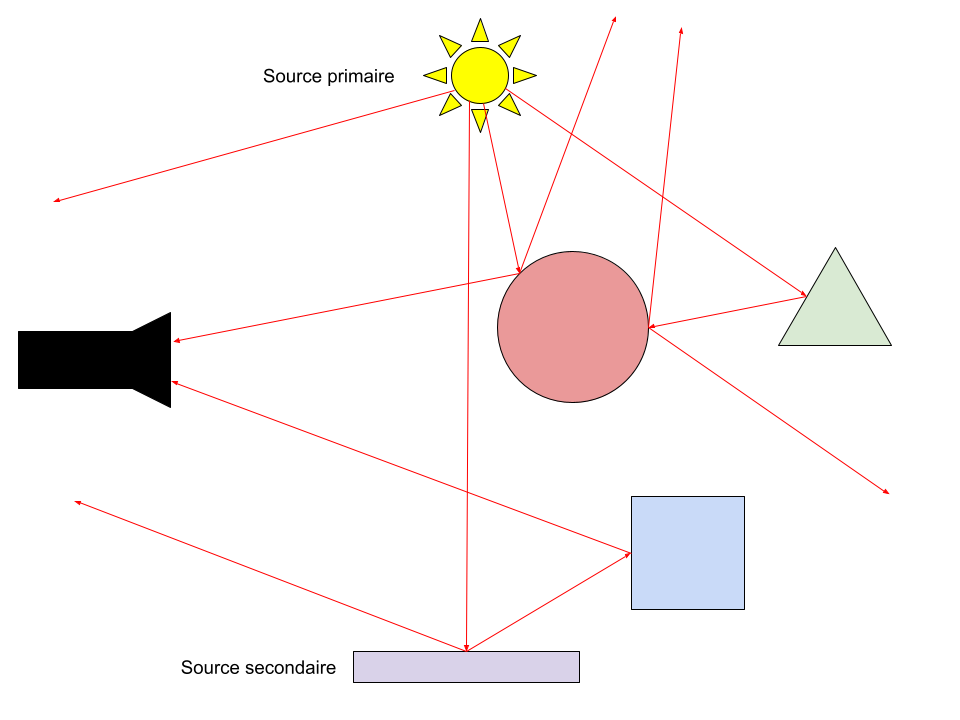
\includegraphics[scale=0.3]{Lumiere.png}
\end{frame}

\begin{frame}
    \frametitle{Principe de Fermat}
    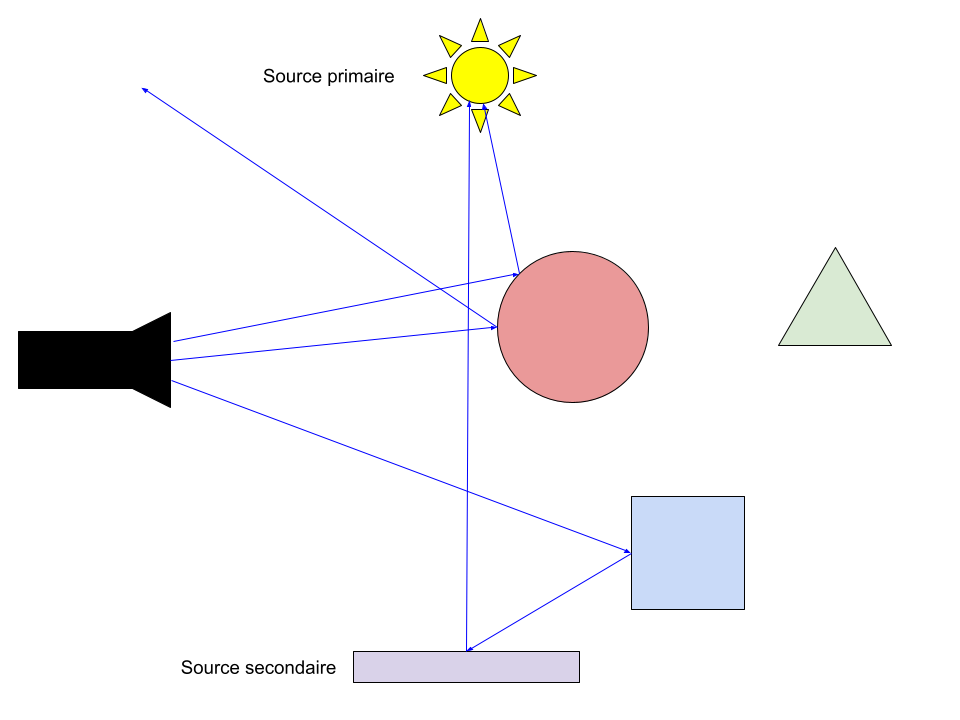
\includegraphics[scale=0.3]{Fermat.png}
\end{frame}

\section{Physicaly based rendering}

\subsection{Radiométrie}

\begin{frame}

    \frametitle{Grandeurs importantes}

    L'énergie $ Q = \frac{hc}{\nu} $ en $ J $.

    La puissance ou flux $ \Phi = \frac{\partial Q}{\partial t} $ en $ W $.

    L'irradiance et l'exitance $ E = \lim_{\Delta A \to 0}  \frac{\Delta \Phi }{\Delta A} $ en $W.m^{-2} $.

    La luminance $ L = \lim_{\Delta \omega \to 0}  \frac{\Delta E }{\Delta \omega } $ en $ W.m^{-2}.sr^{-1} $.
\end{frame}

\begin{frame}

    \frametitle{Equation de rendu}

    \begin{align*}
        L_o(x, \omega_o, \lambda, t)
        &= L_e(x, \omega_o, \lambda, t) \\
        &+ \int_{\Omega}^{} f(x, \omega_i, \omega_0, \lambda, t)
        L_i(x, \omega_i, \lambda, t)
        (\omega_i . n) d\omega_i
    \end{align*}

\end{frame}

\subsection{Types d'interractions}

\begin{frame}

    \frametitle{4 types d'interractions}

    \begin{tabular}{ | c | c | c | }
        \hline
         & \bfseries Réflexion & \bfseries Transmission \\
        \hline
        \bfseries Spéculaire & Réflexion spéculaire & Transparence \\
        \hline
        \bfseries Diffus & Lambertien & Diffusion subsurface \\
        \hline
    \end{tabular}
    
\end{frame}

\subsection{Modéles physiques}

\begin{frame}
    \frametitle{Lambertien}
    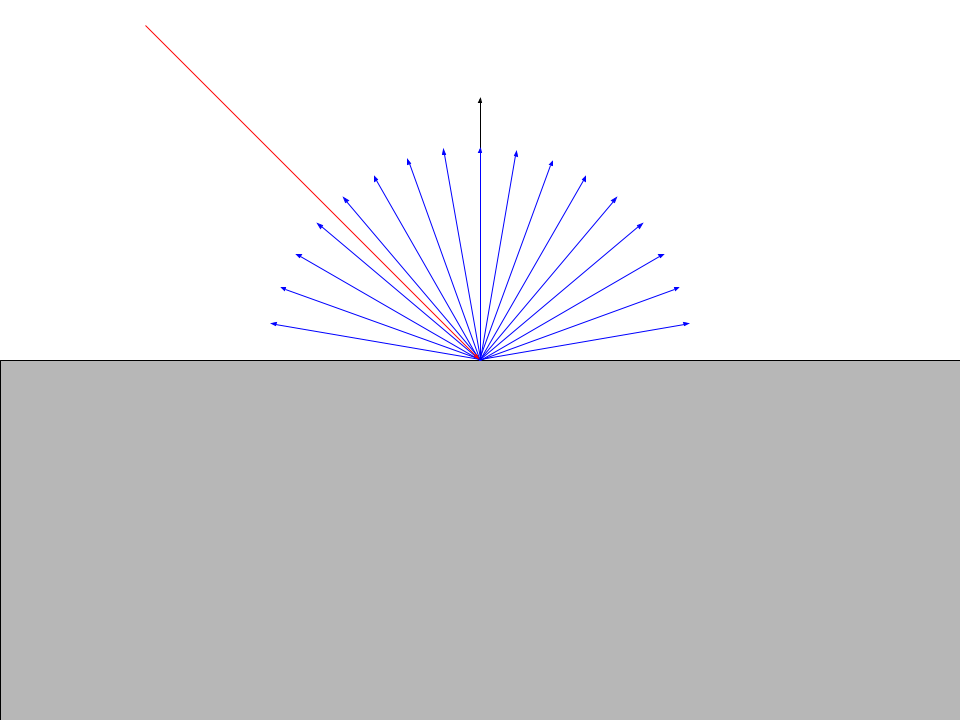
\includegraphics[scale=0.3]{Lambertian.png}
\end{frame}

\begin{frame}
    \frametitle{Réflexion spéculaire}
    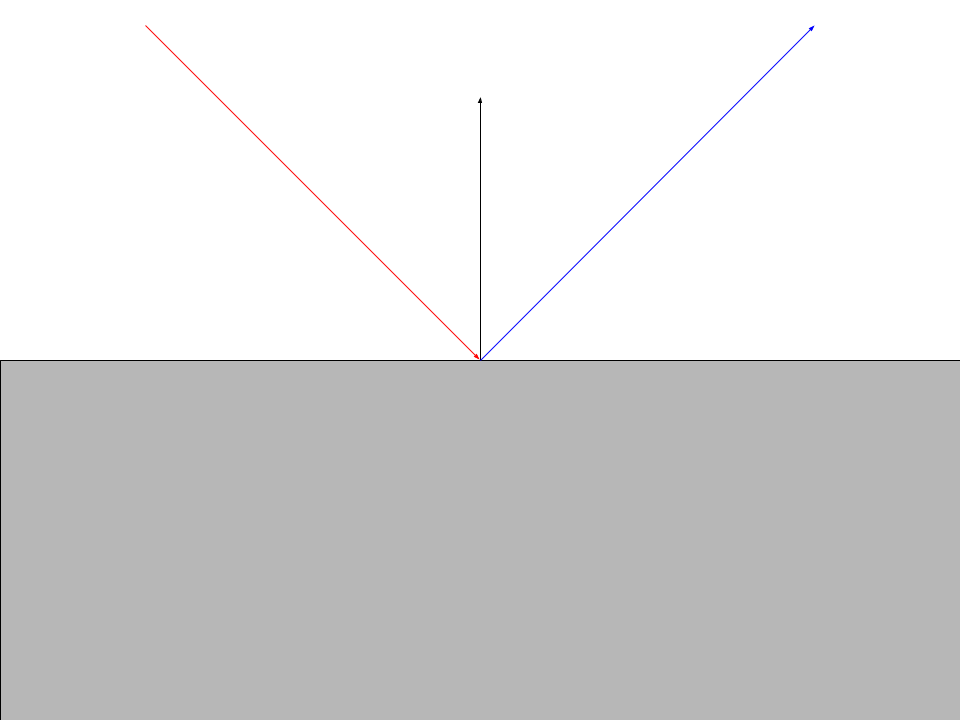
\includegraphics[scale=0.3]{Metal.png}
\end{frame}

\begin{frame}
    \frametitle{Transmission spéculaire}
    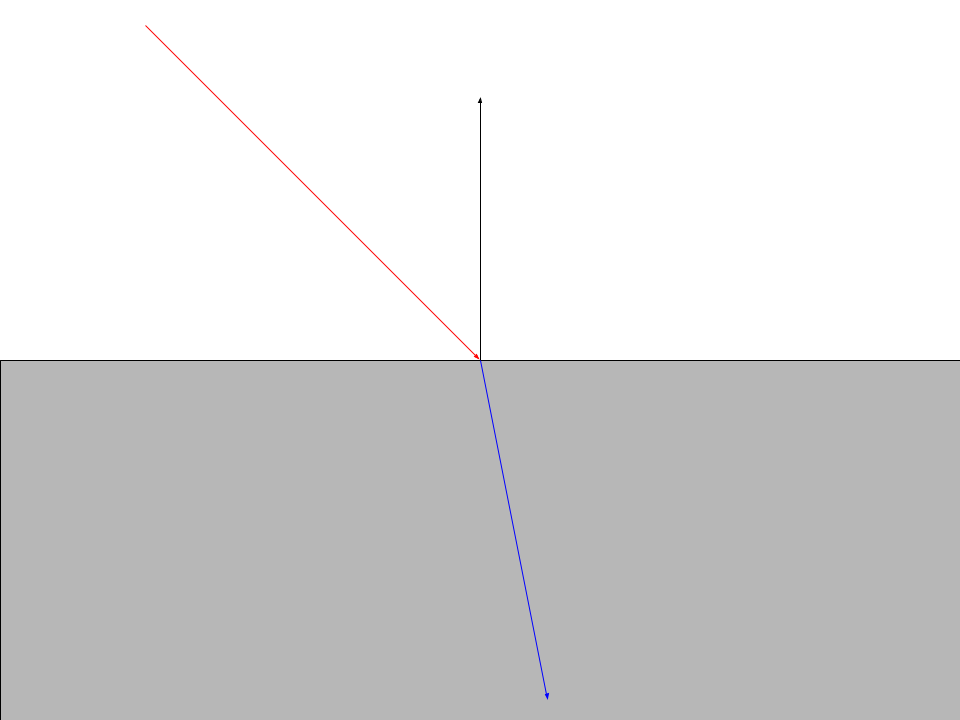
\includegraphics[scale=0.3]{Dielectrique.png}
\end{frame}

\begin{frame}
    \frametitle{Lampe}
    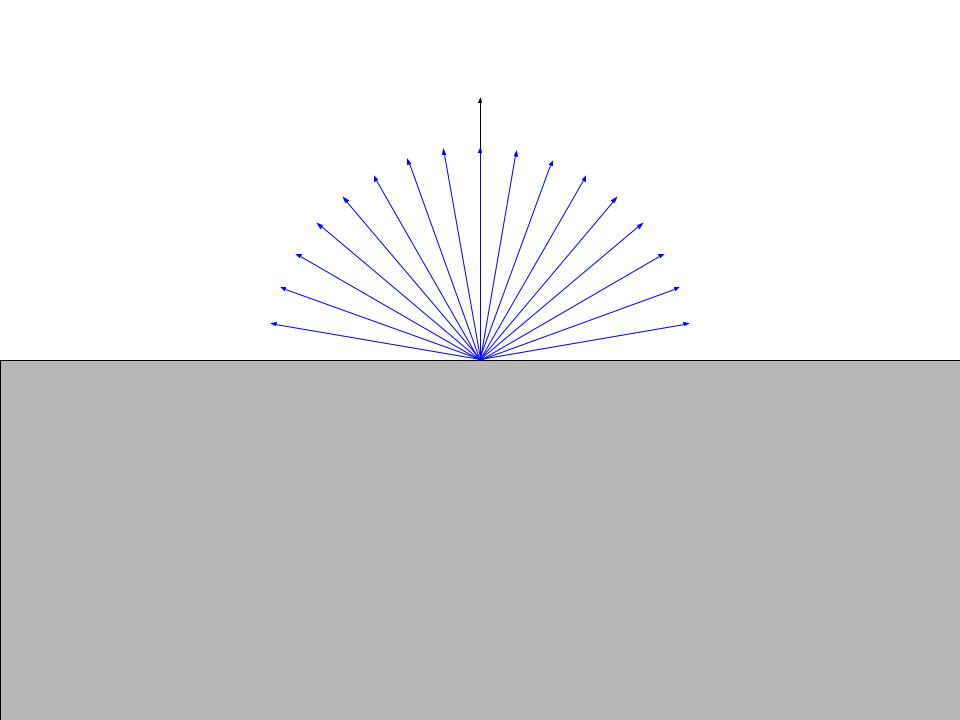
\includegraphics[scale=0.3]{Lampe.png}
\end{frame}

\begin{frame}
    \frametitle{Exemple}
    
\end{frame}

\section{Optimisation}

\subsection{Tests d'intersection}

\begin{frame}
    \frametitle{Bounding Volume Hierarchy (BVH)}
    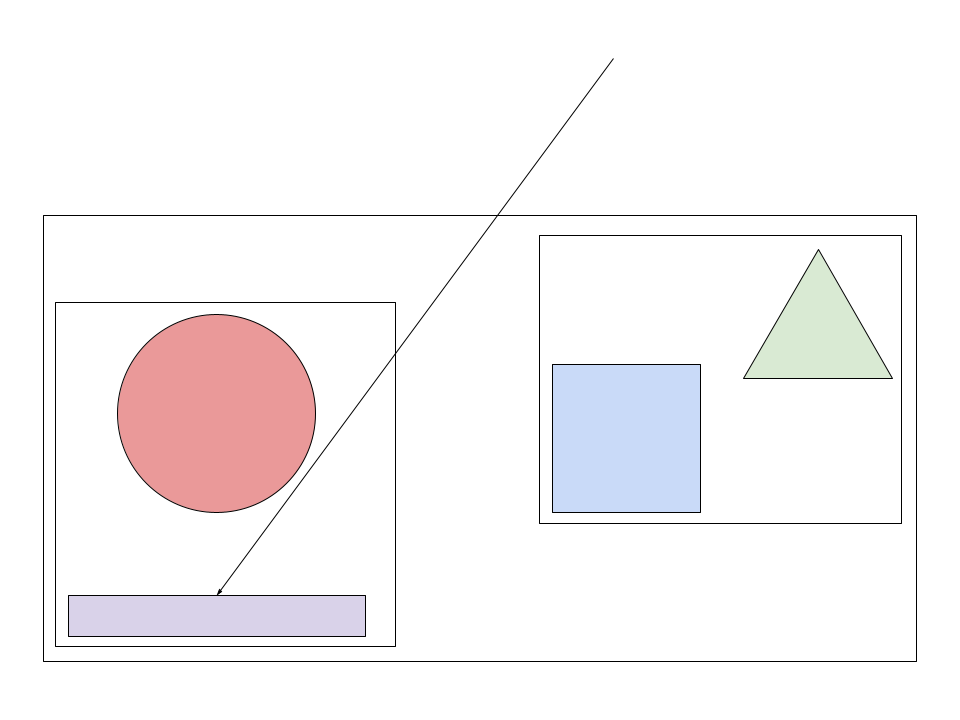
\includegraphics[scale=0.3]{Arbre.png}
\end{frame}

\begin{frame}
    \frametitle{Comparaison}
\end{frame}

\subsection{Priorisation}

\begin{frame}
    \frametitle{Echantillonage d'importance}
    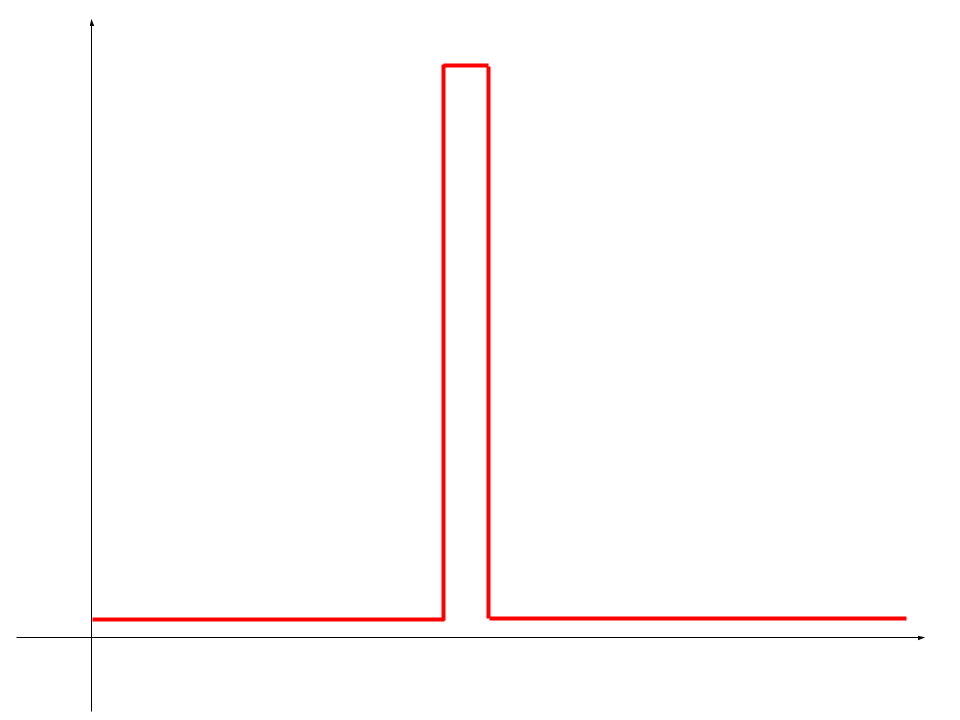
\includegraphics[scale=0.3]{Priorisation.png}
\end{frame}

\begin{frame}
    \frametitle{Comparaison}
\end{frame}

\subsection{Traitement d'image}

\begin{frame}
    \frametitle{Traitement d'image}

    \begin{itemize}
        \item Filtre médian : médiane des pixels voisins.
        \item Filtre gaussien :
            $ G(x,y) = \frac{ e^{ \frac{x^2+y^2}{2 \sigma^2} } }{2 \pi \sigma^2} $.
    \end{itemize}

\end{frame}

\begin{frame}
    \frametitle{Comparaison}
\end{frame}

\end{document}